% questions.tex —— 2019 年·天津卷·理科 · 题目内容片段（无答案）
% 由 tools/generate_projects.py 依来源总账自 2019/2019_数学真题_天津卷理_试题.md 生成，勿手改（改源 MD 后重跑）

\begin{gktip}
来源：固定来源 \texttt{src-6266612a7ec070d21a24172f28c0f92cba14d68bd7f0fe6da69fbb4aeeec1000}（\texttt{普通高考/2019/2019天津理.pdf}，原卷印刷页 1107—1108）。
声明：内部绑定只固定输入字节，不认证出版者、版次、上游来源链及官方身份；固定源不附答案页。
\end{gktip}

\par\medskip

\gkpart{一、选择题（本大题共 8 小题，每小题 5 分，共 40 分。在每小题列出的四个选项中，选出符合题目要求的一项）}

\begin{question}
\gkti{1}
设集合 $A = \{-1, 1, 2, 3, 5\}$, $B = \{2, 3, 4\}$, $C = \{x \in \mathbb{R} \mid 1 \leqslant x < 3\}$, 则 $(A \cap C) \cup B =$（ ）。

(A) $\{2\}$　(B) $\{2, 3\}$　(C) $\{-1, 2, 3\}$　(D) $\{1, 2, 3, 4\}$

\end{question}
\begin{question}
\gkti{2}
\Needspace{5\baselineskip}
设变量 $x, y$ 满足约束条件
\nopagebreak[4]
\[
\begin{cases}
x + y - 2 \leqslant 0, \\
x - y + 2 \geqslant 0, \\
x \geqslant -1, \\
y \geqslant -1,
\end{cases}
\]
则目标函数 $z = -4x + y$ 的最大值为（ ）。

(A) $2$　(B) $3$　(C) $5$　(D) $6$

\end{question}
\begin{question}
\gkti{3}
设 $x \in \mathbb{R}$, 则“$x^2 - 5x < 0$”是“$|x - 1| < 1$”的（ ）。

(A) 充分而不必要条件　(B) 必要而不充分条件  
(C) 充要条件　(D) 既不充分也不必要条件

\Needspace{0.4\textheight}
\end{question}
\begin{question}
\gkti{4}
阅读如图的程序框图, 运行相应的程序, 输出 $S$ 的值为（ ）。
\nopagebreak[4]
\begin{center}\begin{tikzpicture}[>=latex, font=\small, scale=0.9]
  \tikzstyle{startstop} = [draw, rounded corners=6pt, minimum width=1.6cm, minimum height=0.6cm, text centered]
  \tikzstyle{io} = [draw, trapezium, trapezium left angle=70, trapezium right angle=110, minimum width=1.8cm, minimum height=0.6cm, text centered]
  \tikzstyle{process} = [draw, minimum width=2.0cm, minimum height=0.6cm, text centered]
  \tikzstyle{decision} = [draw, diamond, aspect=2.2, minimum width=2.4cm, minimum height=0.7cm, text centered]
  \tikzstyle{arrow} = [thick, ->]

  \node (start) [startstop] at (0, 0) {开始};
  \node (init) [process] at (0, -0.95) {$i = 1,\ S = 0$};
  \node (dec1) [decision] at (0, -2.15) {$i$ 为偶数?};
  \node (proc1) [process] at (0, -3.35) {$j = \dfrac{i}{2}$};
  \node (proc2) [process] at (0, -4.35) {$S = S + i \cdot 2^j$};
  \node (odd) [process] at (2.2, -3.35) {$S = S + i$};
  \node (inc) [process] at (0, -5.35) {$i = i + 1$};
  \node (dec2) [decision] at (0, -6.45) {$i \geqslant 4$?};
  \node (out) [io] at (0, -7.6) {输出 $S$};
  \node (stop) [startstop] at (0, -8.45) {结束};

  \draw[arrow] (start) -- (init);
  \draw[arrow] (init) -- (dec1);
  \draw[arrow] (dec1) -- node[right] {是} (proc1);
  \draw[arrow] (proc1) -- (proc2);
  \draw[arrow] (proc2) -- (inc);
  \draw[arrow] (dec1.east) -| node[above, pos=0.3] {否} (odd.north);
  \draw[arrow] (odd.south) |- ([yshift=0.25cm]inc.north);
  \draw[arrow] (inc) -- (dec2);
  \draw[arrow] (dec2) -- node[right] {是} (out);
  \draw[arrow] (out) -- (stop);

  \draw[arrow] (dec2.west) -- node[above] {否} ++(-1.6, 0) |- ([yshift=0.2cm]dec1.north);
\end{tikzpicture}
\end{center}
\nopagebreak[4]
(A) $5$　(B) $8$　(C) $24$　(D) $29$

\end{question}
\begin{question}
\gkti{5}
已知抛物线 $y^2 = 4x$ 的焦点为 $F$, 准线为 $l$. 若 $l$ 与双曲线 $\dfrac{x^2}{a^2} - \dfrac{y^2}{b^2} = 1$ ($a > 0, b > 0$) 的两条渐近线分别交于点 $A$ 和点 $B$, 且 $|AB| = 4|OF|$ ($O$ 为原点), 则双曲线的离心率为（ ）。

(A) $\sqrt{2}$　(B) $\sqrt{3}$　(C) $2$　(D) $\sqrt{5}$

\end{question}
\begin{question}
\gkti{6}
已知 $a = \log_5 2$, $b = \log_{0.5} 0.2$, $c = 0.5^{0.2}$, 则 $a, b, c$ 的大小关系为（ ）。

(A) $a < c < b$　(B) $a < b < c$　(C) $b < c < a$　(D) $c < a < b$

\end{question}
\begin{question}
\gkti{7}
已知函数 $f(x) = A \sin(\omega x + \varphi)$ ($A > 0, \omega > 0, |\varphi| < \pi$) 是奇函数, 将 $y = f(x)$ 的图象上所有点的横坐标伸长到原来的 $2$ 倍 (纵坐标不变), 所得图象对应的函数为 $g(x)$. 若 $g(x)$ 的最小正周期为 $2\pi$, 且 $g\left(\dfrac{\pi}{4}\right) = \sqrt{2}$, 则 $f\left(\dfrac{3\pi}{8}\right) =$（ ）。

(A) $-2$　(B) $-\sqrt{2}$　(C) $\sqrt{2}$　(D) $2$

\end{question}
\begin{question}
\gkti{8}
已知 $a \in \mathbb{R}$, 设函数 $f(x) = \begin{cases} x^2 - 2ax + 2a, & x \leqslant 1, \\ x - a \ln x, & x > 1, \end{cases}$ 若关于 $x$ 的不等式 $f(x) \geqslant 0$ 在 $\mathbb{R}$ 上恒成立, 则 $a$ 的取值范围为（ ）。

(A) $[0, 1]$　(B) $[0, 2]$　(C) $[0, \mathrm{e}]$　(D) $[1, \mathrm{e}]$

\par\medskip

\end{question}
\gkpart{二、填空题（本大题共 6 小题，每小题 5 分，共 30 分）}

\begin{question}
\gkti{9}
$\mathrm{i}$ 是虚数单位, 则 $\dfrac{5 - \mathrm{i}}{1 + \mathrm{i}}$ 的值为 $\underline{\phantom{XXXX}}$.

\end{question}
\begin{question}
\gkti{10}
$\left(2x - \dfrac{1}{8x^3}\right)^8$ 的展开式中的常数项为 $\underline{\phantom{XXXX}}$.

\end{question}
\begin{question}
\gkti{11}
已知四棱锥的底面是边长为 $\sqrt{2}$ 的正方形, 侧棱长均为 $\sqrt{5}$. 若圆柱的一个底面的圆周经过四棱锥四条侧棱的中点, 另一个底面的圆心为四棱锥底面的中心, 则该圆柱的体积为 $\underline{\phantom{XXXX}}$.

\end{question}
\begin{question}
\gkti{12}
设 $a \in \mathbb{R}$, 直线 $ax - y + 2 = 0$ 和圆 $\begin{cases} x = 2 + 2\cos\theta, \\ y = 1 + 2\sin\theta \end{cases}$ ($\theta$ 为参数) 相切, 则 $a$ 的值为 $\underline{\phantom{XXXX}}$.

\end{question}
\begin{question}
\gkti{13}
设 $x > 0, y > 0, x + 2y = 5$, 则 $\dfrac{(x + 1)(2y + 1)}{\sqrt{xy}}$ 的最小值为 $\underline{\phantom{XXXX}}$.

\end{question}
\begin{question}
\gkti{14}
在四边形 $ABCD$ 中, $AD \parallel BC$, $AB = 2\sqrt{3}$, $AD = 5$, $\angle A = 30^\circ$, 点 $E$ 在线段 $CB$ 的延长线上, 且 $AE = BE$, 则 $\vec{BD} \cdot \vec{AE} =$ $\underline{\phantom{XXXX}}$.

\par\medskip

\end{question}
\gkpart{三、解答题（本大题共 6 小题，共 80 分。解答应写出文字说明、演算步骤或证明过程）}

\begin{question}
\gkti{15}\textbf{（本小题满分 13 分）} 
在 $\triangle ABC$ 中, 内角 $A, B, C$ 所对的边分别为 $a, b, c$. 已知 $b + c = 2a$, $3c \sin B = 4a \sin C$.
(1) 求 $\cos B$ 的值;
(2) 求 $\sin\left(2B + \dfrac{\pi}{6}\right)$ 的值.

\end{question}
\begin{question}
\gkti{16}\textbf{（本小题满分 13 分）} 
设甲、乙两位同学上学期间, 每天 7:30 之前到校的概率均为 $\dfrac{2}{3}$. 假定甲、乙两位同学到校情况互不影响, 且任一同学每天到校情况相互独立.
(1) 用 $X$ 表示甲同学上学期间的三天中 7:30 之前到校的天数, 求随机变量 $X$ 的分布列和数学期望;
(2) 设 $M$ 为事件“上学期间的三天中, 甲同学在 7:30 之前到校的天数比乙同学在 7:30 之前到校的天数恰好多 2”, 求事件 $M$ 发生的概率.

\Needspace{0.4\textheight}
\end{question}
\begin{question}
\gkti{17}\textbf{（本小题满分 13 分）} 
如图, $AE \perp \text{\text{平面} } ABCD$, $CF \parallel AE$, $AD \parallel BC$, $AD \perp AB$, $AB = AD = 1$, $AE = BC = 2$.
\nopagebreak[4]
\begin{center}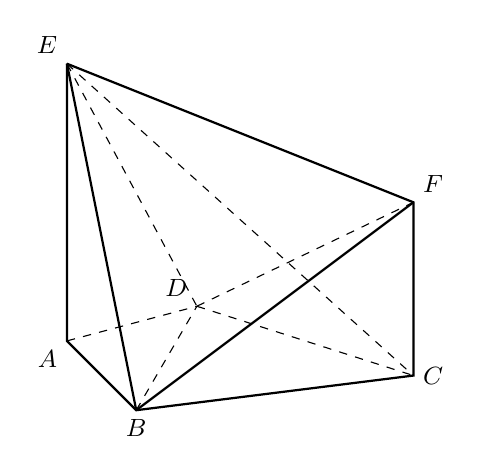
\begin{tikzpicture}[>=latex, font=\small, scale=1.1]
  % 顶点坐标
  \coordinate (A) at (0, 0);
  \coordinate (B) at (0.8, -0.8);
  \coordinate (C) at (4.0, -0.4);
  \coordinate (D) at (1.5, 0.4);
  \coordinate (E) at (0, 3.2);
  \coordinate (F) at (4.0, 1.6);

  % 虚线不可见边/内部对角线
  \draw[dashed, thin] (A) -- (D);
  \draw[dashed, thin] (D) -- (C);
  \draw[dashed, thin] (E) -- (D);
  \draw[dashed, thin] (E) -- (C);
  \draw[dashed, thin] (B) -- (D);
  \draw[dashed, thin] (D) -- (F);

  % 实线可见外轮廓与面边界
  \draw[thick] (E) -- (A) -- (B) -- (C) -- (F) -- (E);
  \draw[thick] (E) -- (B);
  \draw[thick] (B) -- (F);

  % 顶点标记
  \node[above left] at (E) {$E$};
  \node[below left] at (A) {$A$};
  \node[below] at (B) {$B$};
  \node[right] at (C) {$C$};
  \node[above right] at (F) {$F$};
  \node[above left] at (D) {$D$};
\end{tikzpicture}
\end{center}
\nopagebreak[4]
(1) 求证: $BF \parallel \text{\text{平面} } ADE$;
(2) 求直线 $CE$ 与平面 $BDE$ 所成角的正弦值;
(3) 若二面角 $E - BD - F$ 的余弦值为 $\dfrac{1}{3}$, 求线段 $CF$ 的长.

\end{question}
\begin{question}
\gkti{18}\textbf{（本小题满分 13 分）} 
设椭圆 $\dfrac{x^2}{a^2} + \dfrac{y^2}{b^2} = 1$ ($a > b > 0$) 的左焦点为 $F$, 上顶点为 $B$. 已知椭圆的短轴长为 $4$, 离心率为 $\dfrac{\sqrt{5}}{5}$.
(1) 求椭圆的方程;
(2) 设点 $P$ 在椭圆上, 且异于椭圆的上、下顶点, 点 $M$ 为直线 $PB$ 与 $x$ 轴的交点, 点 $N$ 在 $y$ 轴的负半轴上. 若 $|ON| = |OF|$ ($O$ 为原点), 且 $OP \perp MN$, 求直线 $PB$ 的斜率.

\end{question}
\begin{question}
\gkti{19}\textbf{（本小题满分 14 分）} 
设 $\{a_n\}$ 是等差数列, $\{b_n\}$ 是等比数列. 已知 $a_1 = 4, b_1 = 6, b_2 = 2a_2 - 2, b_3 = 2a_3 + 4$.
(1) 求 $\{a_n\}$ 和 $\{b_n\}$ 的通项公式;
(2) 设数列 $\{c_n\}$ 满足 $c_1 = 1$, $c_n = \begin{cases} 1, & 2^k < n < 2^{k+1}, \\ b_k, & n = 2^k, \end{cases}$ 其中 $k \in \mathbb{N}^*$.
① 求数列 $\{a_{2^n}(c_{2^n} - 1)\}$ 的通项公式;
② 求 $\sum_{i=1}^{2^n} a_i c_i$ ($n \in \mathbb{N}^*$).

\end{question}
\begin{question}
\gkti{20}\textbf{（本小题满分 14 分）} 
设函数 $f(x) = \mathrm{e}^x \cos x$, $g(x)$ 为 $f(x)$ 的导函数.
(1) 求 $f(x)$ 的单调区间;
(2) 当 $x \in \left[\dfrac{\pi}{4}, \dfrac{\pi}{2}\right]$ 时, 证明 $f(x) + g(x)\left(\dfrac{\pi}{2} - x\right) \geqslant 0$;
(3) 设 $x_n$ 为函数 $u(x) = f(x) - 1$ 在区间 $\left(2n\pi + \dfrac{\pi}{4}, 2n\pi + \dfrac{\pi}{2}\right)$ 内的零点, 其中 $n \in \mathbb{N}$, 证明 $2n\pi + \dfrac{\pi}{2} - x_n < \dfrac{\mathrm{e}^{-2n\pi}}{\sin x_0 - \cos x_0}$.

\end{question}